\section{Strings}

\index{string.h}

The C Programming Language doesn't have a specific type dedicated for strings. Instead it makes use of \textit{char arrays} to represent a string. A string is defined as an array of characters (char's) terminated by a char value 0. In other words, a string is simply an one-dimensional array of char's which has an extra element at the end set to 0. 

In this section we will cover three common string functions which are available, but note there are many more string functions available.

\begin{figure}[H]
\centerline{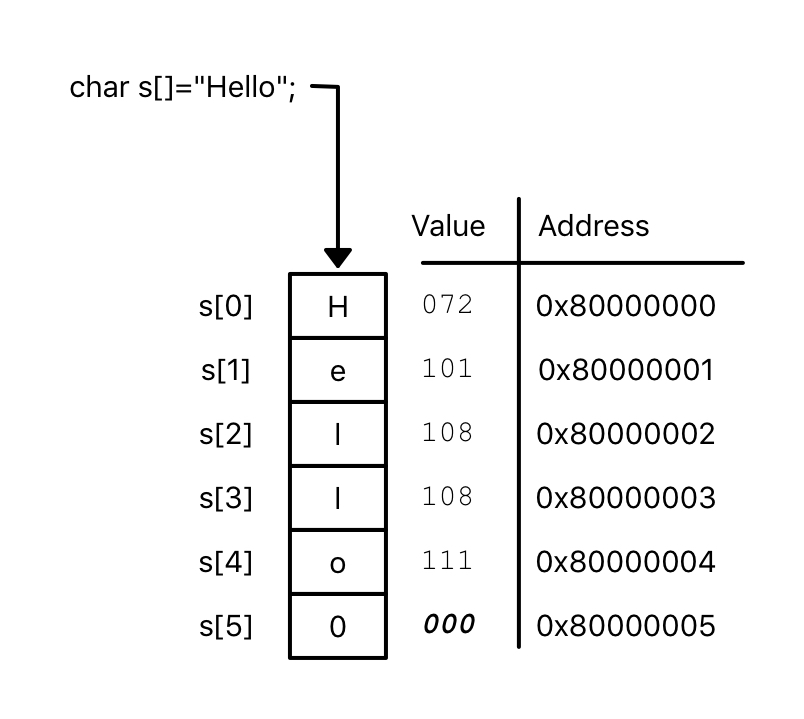
\includegraphics[width=0.6\textwidth]{string.jpg}}
\caption{"Hello" string as a char array}
\label{HelloString}
\end{figure}

The figure \ref{HelloString} shows the "Hello" string represented in memory. The last location in the array s[5] contains 0 which terminates the string. If we calculate the entire length of the string it is 5 ("Hello") + 1 (0, Terminator) which is 6 and not 5.  

\subsection{strlen(...)}

\index{strlen(...)}

The function \textit{strlen(...)} returns the length of a string but unfortunately it returns the length without the 0 terminator. It is important when defining a string to include the 0 terminator within the calculation. The compiler will allocate the right amount of space when compiling but the code itself has to take into account the additional string terminator.

\begin{lstlisting}[language=C,showstringspaces=false,caption={File: strlen.c},label={strcmp},captionpos=b,label=strlen]

 1 #include <stdio.h>
 2 #include <string.h>
 3    
 4 int main(void)
 5 {
 6 char str1[] = "Hello";
 7 
 8 printf("... string length \"Hello\"   = %lu\n",strlen(str1));
 9 printf("... string length \"Hello\"+0 = %lu\n",strlen(str1)+1);
10  
11 return 0;
12 }

INTERACTION

$ cc strlen.c
$ ./a.out
... string length "Hello"   = 5
... string length "Hello"+0 = 6
$

\end{lstlisting}

Listing \ref{strlen} shows the forming of a string and then obtaining the string length. Line:6 shows a string being formed. The array doesn't have a fixed size [], this number is provided by the compiler. Line:8 outputs the \textit{strlen(...)} function which shows that it only provides the length of the string without the terminator. Line:9 adds the 0 terminator to the string length.

\subsection{strcmp(...)}

\index{strcmp(...)}

Similar to many programming languages, string comparisons are treated slightly differently from the general mathematical comparisons i.e. ==. In C a function such as \textit{strcmp(...)} is used to carry out a string comparison. This function can be found in the \textit{string.h} standard library. 

\begin{lstlisting}[language=C,showstringspaces=false,caption={File: strcmp.c},label={strcmp},captionpos=b]

 1 #include <stdio.h>
 2 #include <string.h>
 3 
 4 int main(void)
 5 {
 6 char str1[] = "abcdefg";
 7 char str2[] = "12345";
 8 
 9   if (!strcmp(str1,"abcdefg"))
10     printf("... 1 str1 equal to \"abcdefg\" \n");
11   else
12     printf("... 1 str1 not equal to \"abcdefg\" \n");
13 
14   if (!strcmp(str1,str2))
15     printf("... 2 str1 equal to str2 \n");
16   else
17     printf("... 2 str1 not equal to str2 \n");
18 
19 return 0;
20 }

INTERACTION

$ cc strcmp.c
$ ./a.out
... 1 str1 equal to "abcdefg" 
... 2 str1 not equal to str2 
$

\end{lstlisting}

Listing \ref{strcmp} shows an example of using \textit{strcmp}. The code carries out two comparisons. The first tests to see if \textit{str1} is equal to the fixed string "abcdefg", as shown on line:9. The second test checks whether two string arrays are the same, as shown on line:14. The first should be true and the second should be false.

\subsection{strcpy(...)}

\index{strcpy(...)}

The \textit{strcpy(...)} function copies a source string to a destination string and returns a pointer to the destination string. The important part is that the destination string points to enough memory to contain a copy of the source string. In other words care has to be taken to make sure there is sufficient memory for the copy. If insufficient memory is allocated for the destination string then a program can become corrupt, as data overwrites either variables or code.  

Corruption leads to instability. These errors are difficult to track down, as they tend to emerge in different forms. The C compiler does not provide any assistance in identifying these types of errors. It is the responsibility of the programmer.  

\begin{lstlisting}[language=C,showstringspaces=false,caption={File: strcpy.c},captionpos=b,label=strcpy]

 1 #include <stdio.h>
 2 #include <string.h>
 3   
 4 int main (void)
 5 {
 6 char src[] = "Hello";
 7 char dest[10];
 8   
 9 printf ("dest \"%s\" == src \"%s\"\n",strcpy(dest,src),src);
10 
11 return 0;
12 }

INTERACTION

$ cc strcpy.c
$ ./a.out
dest "Hello" == src "Hello"
$

\end{lstlisting}

Listing \ref{strcpy} shows a string copy. The destination string \textit{dest[10]} has a fixed length of 10 characters and the source string \textit{src[6]} has a fixed length of 6 characters allocated. The \textit{strcpy(...)} function on line:9 returns a pointer to the destination string. This string is then used  by the \textit{printf(...)} to output the result of the function.
  
 
